We illustrate the \pkg{parfm} package with the very well-known \code{kidney} dataset 
  that contains the recurrence times to kidney infection for 38 patients using portable dialysis equipment \citep{McGilchristAisbett91}.
\begin{CodeChunk}
\begin{CodeInput}
R> R.Version()[["version.string"]]
\end{CodeInput}
\begin{CodeOutput}
[1] "R version 3.3.1 (2016-06-21)"
\end{CodeOutput}
\begin{CodeInput}
R> library("parfm")
R> packageDescription("parfm", fields="Version")
\end{CodeInput}
\begin{CodeOutput}
[1] "2.7"
\end{CodeOutput}
\end{CodeChunk}
The dataset is available in \pkg{parfm} via the command \code{data("kidney")} and it looks like the following:
\begin{CodeChunk}
\begin{CodeInput}
R> head(kidney)
\end{CodeInput}
\begin{CodeOutput}
  id time status age sex disease frail
1  1    8      1  28   1   Other   2.3
2  1   16      1  28   1   Other   2.3
3  2   23      1  48   2      GN   1.9
4  2   13      0  48   2      GN   1.9
5  3   22      1  32   1   Other   1.2
6  3   28      1  32   1   Other   1.2
\end{CodeOutput}
\end{CodeChunk}

Each observation corresponds to a kidney, 
  the variable \code{id} being the patient's code.
The time from insertion of the catheter to infection or censoring is stored in \code{time}
  while \code{status} is 1 when infection has occurred and 0 for censored observations (catheters may be removed for reasons other than infection).
Three covariates are available: \code{age}, the age of the patient in years,
  \code{sex}, being \code 1 for males and \code 2 for females,
  and \code{disease}, the disease type
  (\code{GN}, \code{AN}, \code{PKD} or \code{Other}).
Finally \code{frail} is the frailty prediction from the original paper which fits a semi-parametric lognormal frailty model.

First and foremost, \code{sex} is recoded as a 0--1 indicator for ease of interpretation:
\begin{CodeChunk}
\begin{CodeInput}
R> kidney$sex <- kidney$sex - 1
\end{CodeInput}
\end{CodeChunk}

The hazard of infection will be modelled as a function of the patient's age and sex.
Clearly, kidneys from the same patient cannot be considered independent.
Therefore, the use of a shared frailty model is advisable, with clusters of size 2 corresponding to patients.

The \code{parfm()} function must have the following inputs.
    \code{formula}: a formula with an object of class \code{Surv} on the left-hand side;
    \code{cluster}: the cluster variable's name; 
    \code{data}: the dataset;
    \code{dist}: the baseline hazard,
      either \code{exponential}, \code{weibull}, \code{gompertz}, \code{lognormal} or \code{loglogistic};
    \code{frailty}: the frailty distribution,
      either \code{none}, \code{gamma}, \code{possta} or \code{ingau}.
  
\paragraph{Model estimation.}
The model with exponential baseline hazard and gamma frailty distribution is first fitted.

\begin{CodeChunk}
\begin{CodeInput}
R> mod <- parfm(Surv(time, status) ~ sex + age, cluster="id", 
+               data=kidney, dist="exponential", frailty="gamma")
R> mod
\end{CodeInput}
\begin{CodeOutput}
Frailty distribution: Gamma 
Basline hazard distribution: Exponential 
Loglikelihood: -333.248 

       ESTIMATE SE    p-val    
theta   0.301   0.157          
lambda  0.025   0.015          
sex    -1.485   0.398 <.001 ***
age     0.005   0.011 0.662    
---
Signif. codes: 0 '***' 0.001 '**' 0.01 '*' 0.05 '.' 0.1 ' ' 1

Kendall's Tau: 0.131 
\end{CodeOutput}
\end{CodeChunk}

Standard errors are computed as the square roots of the diagonal elements of the observed information matrix.
According to this model, \code{sex} has a significant impact on the hazard of infection 
  while it is not affected by \code{age}. 
Conditional on the patient's frailty and on the age, 
  the hazard of infection for a female at any time $t$ is estimated to be 
  $\exp(-1.485) \approx 0.227$ times that of a male,
  with Wald confidence interval  
\begin{CodeChunk}
\begin{CodeInput}
> ci.parfm(mod, level=0.05)["sex",]
\end{CodeInput}
\begin{CodeOutput}
  low    up 
0.104 0.495 
\end{CodeOutput}
\end{CodeChunk}
% (IC: $0.104$ -- $0.495$). 
As for the heterogeneity parameter, it is estimated to be $0.301$ which corresponds to a Kendall's tau equal to $0.131$.

% % % % % % % % % % % % % % % % % % % % % % % Prediction % % % % % % % % % % % % % % % % % % % % % % %
\paragraph{Frailty prediction.}
Prediction of frailties can be obtained via the \code{predict()} function, with the parametric frailty model
  object as unique argument.
For instance, the predictions for the gamma--exponential model, \code{mod}, are obtained via the command
\begin{CodeChunk}
\begin{CodeInput}
R> u <- predict(mod)
\end{CodeInput}
\end{CodeChunk}
which returns an object of class \code{predict.parfm}.
These predictions can easily be plotted (Figure~\ref{fig:kidney.prediction}) with the command \code{plot(u, sort="i")}.
\begin{figure}[ht]
  \centering
  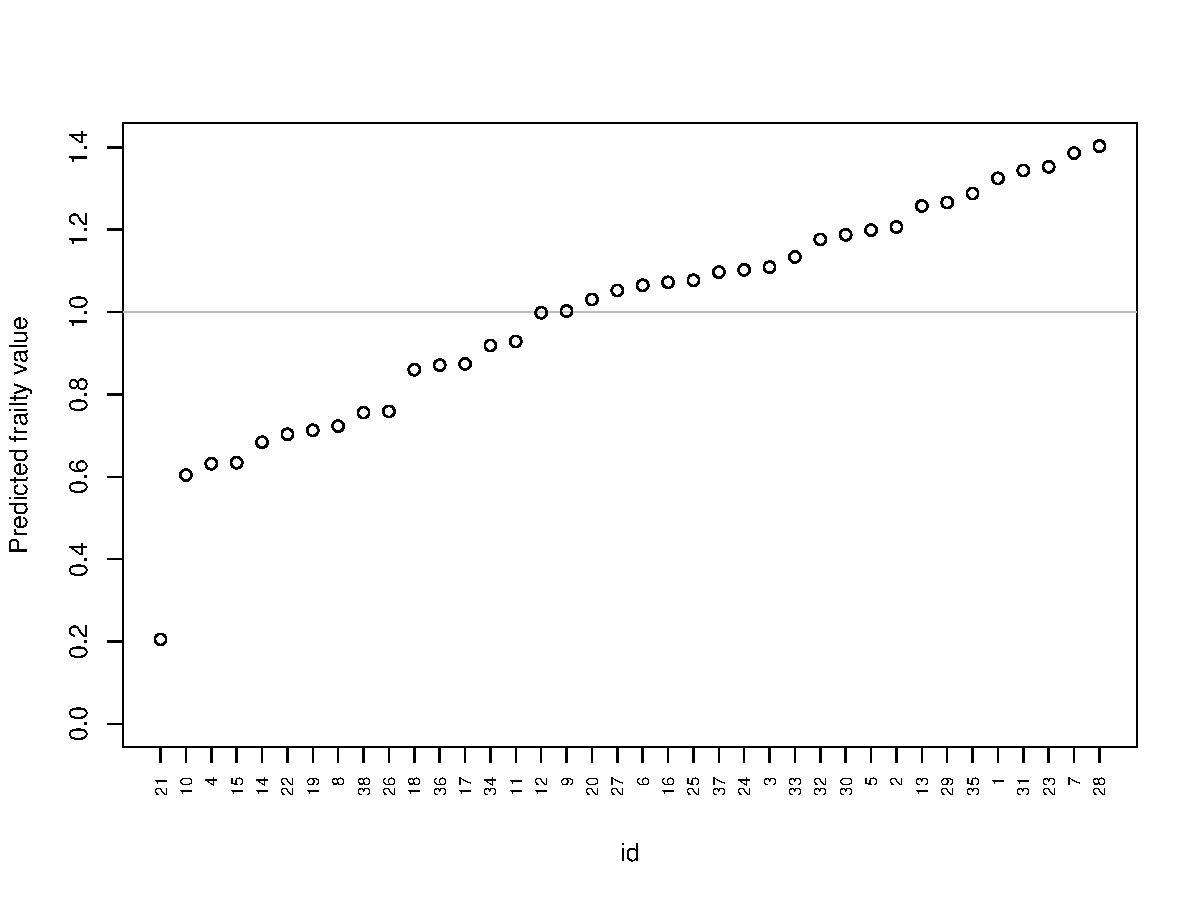
\includegraphics[width=.95\textwidth]{./graphs/prediplot.pdf}
  \caption{Prediction of frailties for the {kidney} dataset
    as given by the parametric gamma--exponential frailty model.}
  \label{fig:kidney.prediction}
\end{figure}


% % % % % % % % % % % % % % % % % % Comparison of different models % % % % % % % % % % % % % % % % % %
\paragraph{Comparison of different models.}
In some circumstances, it might be useful to easily obtain AIC and BIC values 
  for a series of candidate models. 
  This can be done using the \code{select.parfm()} function.
% The \code{select.parfm()} function is used to obtain the AIC and BIC for all candidate models.
% Even though, in clinical practice, a parametric form is assumed only in presence of strong previous information,
% \todo{ Is it clear that this is not a standard way to choose a model?}
%   this tool might help in the choice of the model.
Its use is similar to that of the \code{parfm()} function,
  but the \code{dist} and \code{frailty} values are vectors
  that contain all the alternatives to try.

\begin{CodeChunk}
\begin{CodeInput}
R> kidney.parfm <- select.parfm(Surv(time, status) ~ sex + age, 
+    cluster="id", data=kidney,
+    dist=c("exponential", "weibull", "loglogistic",
+           "lognormal", "logskewnormal"),
+    frailty=c("gamma", "ingau", "possta", "lognormal"))
R> kidney.parfm
\end{CodeInput}
\begin{CodeOutput}
 AIC:             gamma  ingau possta lognor
   exponential      674    676    682    675
   weibull          674    677    682    676
   loglogistic      685    685    686    685
   lognormal        679    679    681    679
   logskewnormal    681    681    682    681

 BIC:             gamma  ingau possta lognor
   exponential      684    685    692    685
   weibull          686    688    694    687
   loglogistic      697    697    697    696
   lognormal        691    691    692    691
   logskewnormal    695    695    696    695
\end{CodeOutput}
\end{CodeChunk}

\begin{figure}
  \centering
  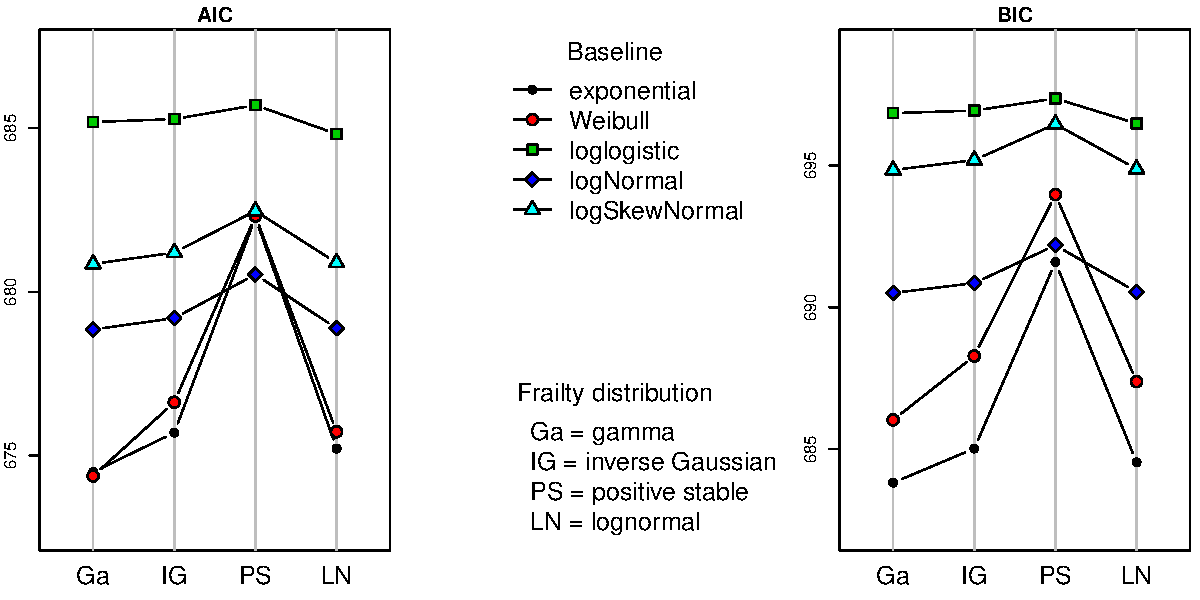
\includegraphics[width=.95\textwidth]{./graphs/plot.pdf}
  \caption{AIC and BIC values of \pkg{parfm} models for the {kidney} dataset.}
  \label{fig:kidney.parfm}
\end{figure}

The results can be plotted (Figure~\ref{fig:kidney.parfm}) via the command \code{plot(kidney.parfm)}.
In this particular example, the exponential baseline seems to be a good candidate.

As a comparison, the model with inverse Gaussian distributed frailties
  is fitted by changing the \code{frailty} argument into \code{`ingau'}.

\begin{CodeChunk}
\begin{CodeInput}
R> parfm(Surv(time, status) ~ sex + age, cluster="id", 
+        data=kidney, dist="exponential", frailty="ingau")
\end{CodeInput}
\begin{CodeOutput}
Frailty distribution: Inverse Gaussian 
Basline hazard distribution: Exponential 
Loglikelihood: -333.85 

       ESTIMATE SE    p-val    
theta   0.375   0.259          
lambda  0.022   0.013          
sex    -1.310   0.373 <.001 ***
age     0.004   0.011 0.693    
---
Signif. codes: 0 '***' 0.001 '**' 0.01 '*' 0.05 '.' 0.1 ' ' 1

Kendall's Tau: 0.125 
\end{CodeOutput}
\end{CodeChunk}

In this case, the conclusions drawn from the previous two models are essentially analogous.

Consider now the model with the positive stable frailty distribution.
In this example, it converges to a solution which is not valid ($\nu=0$)
  with the default settings.

\begin{CodeChunk}
\begin{CodeInput}
R> parfm(Surv(time, status) ~ sex + age, cluster="id", 
+        data=kidney, dist="exponential", frailty="possta")
\end{CodeInput}
\begin{CodeOutput}
Frailty distribution: Positive Stable 
Basline hazard distribution: Exponential 
Loglikelihood: -337.132 

       ESTIMATE SE p-val 
nu      0.000            
lambda  0.012            
sex    -0.885            
age     0.004            
---
Signif. codes: 0 '***' 0.001 '**' 0.01 '*' 0.05 '.' 0.1 ' ' 1

Kendall's Tau: 0 
Warning message:
In parfm(Surv(time, status) ~ sex + age, cluster = "id", data = kidney,  :
  Error in solve.default(res$hessian) : 
  Lapack routine dgesv: system is exactly singular
\end{CodeOutput}
\end{CodeChunk}

The default initial value for $\nu$ is $1/2$ in the case of positive stable frailties;
 it can be changed by means of the \code{iniFpar} option in \code{parfm()}.
Let us try with $\nu= 0.25$.

\begin{CodeChunk}
\begin{CodeInput}
R> parfm(Surv(time, status) ~ sex + age, cluster="id", 
+        data=kidney, dist="exponential", frailty="possta", 
+        iniFpar=0.25)
\end{CodeInput}
\begin{CodeOutput}
Execution time: 1.71 second(s)

Frailty distribution: Positive Stable 
Basline hazard distribution: Exponential 
Loglikelihood: -336.182 

       ESTIMATE SE    p-val    
nu      0.112   0.084          
lambda  0.014   0.008          
sex    -0.951   0.348 0.006 ** 
age     0.004   0.011 0.698    
---
Signif. codes: 0 '***' 0.001 '**' 0.01 '*' 0.05 '.' 0.1 ' ' 1

Kendall's Tau: 0.112 
\end{CodeOutput}
\end{CodeChunk}

The problem might also be fixed by changing the optimisation method (see \code{optim()}).
By default it is set to \code{`BFGS'}, 
  but it can be changed through the \code{method} option.

\begin{CodeChunk}
\begin{CodeInput}
R> parfm(Surv(time, status) ~ sex + age, cluster="id", 
+        data=kidney, dist="exponential", frailty="possta", 
+        method="Nelder-Mead")
\end{CodeInput}
\begin{CodeOutput}
Execution time: 1.51 second(s)

Frailty distribution: Positive Stable 
Basline hazard distribution: Exponential 
Loglikelihood: -336.182 

       ESTIMATE SE    p-val    
nu      0.112   0.084          
lambda  0.014   0.008          
sex    -0.951   0.348 0.006 ** 
age     0.004   0.011 0.694    
---
Signif. codes: 0 '***' 0.001 '**' 0.01 '*' 0.05 '.' 0.1 ' ' 1

Kendall's Tau: 0.112 
\end{CodeOutput}
\end{CodeChunk}

In this example the results obtained by changing the optimisation method are the same
  as those obtained by changing the initial value of $\nu$.
When convergence problems occur, using different starting values and/or different optimisation methods
  is generally sufficient to find the global maximum of the marginal likelihood function.


  
% % % Semiparametric model
Finally we provide a comparison with the semi-parametric model.
As an example, we fit the semi-parametric model with gamma frailties via the \code{coxph()} function.
\begin{CodeChunk}
\begin{CodeInput}
R> coxph(Surv(time, status) ~ sex + age +
+        frailty(id, distribution="gamma", eps=1e-11),
+        outer.max=15, data=kidney)
\end{CodeInput}
\begin{CodeOutput}
                         coef     se(coef) se2    Chisq DF   p      
sex                       -1.58323 0.4594   0.3515 11.88  1.0 0.00057
age                        0.00522 0.0119   0.0088  0.19  1.0 0.66000
frailty(id, distribution                           22.96 12.9 0.04100

     Variance of random effect= 0.408   I-likelihood = -181.6 
\end{CodeOutput}
\end{CodeChunk}

Estimates of regression parameters are quite similar to those of the exponential--gamma model,
  while the frailty variance is sensibly different,
  arguably because of the difference in how the baseline hazard is treated.
